Анализ естественного языка это межпредметная дисциплина, включающая теорию алгоритмов, 
лингвистику и машинное обучение.

\begin{figure}[h]
    \centering
    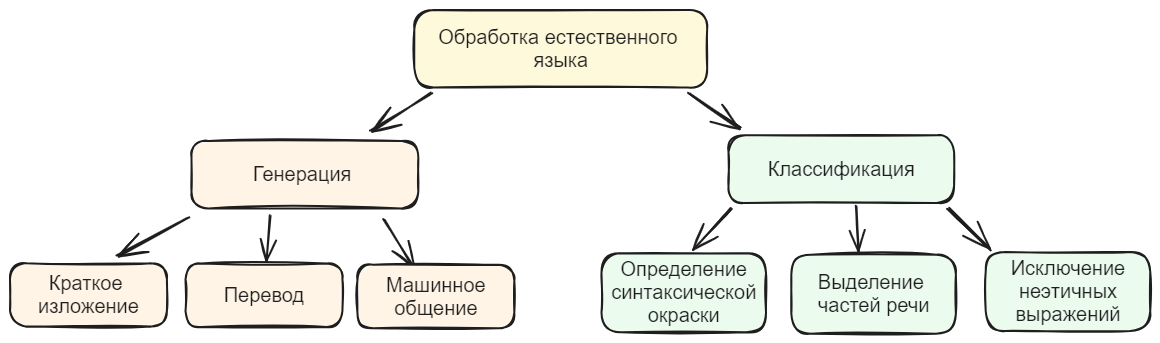
\includegraphics[width=0.5\textwidth]{assets/ml/nlp/taxonomy.excalidraw.png}
    \caption{Таксономия современных подходов обработки естественного языка}
    \label{llm_taxonomy}
\end{figure}

Формальные языки широко используются в математике, логике, лингвистике и компьютерных науках. 
В программировании, например, формальные языки включают языки программирования и описания данных, 
где синтаксис строго определён для обеспечения корректности и предсказуемости выполнения программ.

особенно важным для развития генеративного моделирования.
В областях обработки естественного языка стала популярна аналитическая форма механизма внимания \cite{vaswani2017attention},
приведшая к созданию больших лингвистических моделей \cite{radford2019language}, имеющих важное практическое применение.

